% ==========================================
% CHAPITRE 6 — CORRIGÉ SELON RAPPORT DE JURY
% ==========================================
\newpage
\chapter{ÉTUDE DU SPRINT 4}


\vspace{2.5cm}

\noindent \textbf{\Large Plan}
\vspace{0.8cm}

\begin{enumerate}[label=\textbf{\arabic*}, leftmargin=1.5cm, labelsep=0.8cm]
    \item[] \hspace*{-1.5cm}\textbf{Introduction}                              \dotfill \pageref{sec:s4-intro}
    \item \textbf{User Stories du quatrième sprint}          \dotfill \pageref{sec:s4-userstories}
    \item \textbf{Backlog du quatrième Sprint}               \dotfill \pageref{sec:s4-backlog}
    \item \textbf{Spécification fonctionnelle du Sprint 4}   \dotfill \pageref{sec:s4-specification}
    \item \textbf{Conception du Sprint 4}                    \dotfill \pageref{sec:s4-conception}
    \item \textbf{Étude et réalisation du Sprint 4}          \dotfill \pageref{sec:s4-realisation}
    \item \textbf{Tests et Validation}                       \dotfill \pageref{sec:s4-tests}
    \item \textbf{Rituels Agiles et Clôture du Sprint}       \dotfill \pageref{sec:s4-rituels}
    \item[] \hspace*{-1.5cm} \textbf{Conclusion}                                \dotfill \pageref{sec:s4-conclusion}
\end{enumerate}

\vfill
\newpage

% ============================================================
\section*{Introduction}
\label{sec:s4-intro}
\addcontentsline{toc}{section}{Introduction}
% ============================================================

S'appuyant sur les acquis du Sprint 3 (moteur de paie et gestion des congés),
 ce chapitre présente les réalisations du quatrième et dernier sprint.
  Ce sprint finalise la plateforme PaieZone RH en intégrant la gestion 
  comptable (export SAGE), la conformité réglementaire (CNSS, CAVIS, IRPP), 
  la production de documents administratifs, et l'assistant conversationnel
   PaieBot, basé sur Ollama/phi3 avec architecture RAG et pipeline Text-to-SQL.
    La démarche agile (User Stories, modélisation UML, conception technique,
     interfaces Angular, tests et clôture) a été maintenue.

% ============================================================
\section{User Stories du quatrième sprint}
\label{sec:s4-userstories}
% ============================================================

Lors de la réunion de planification du Sprint 4, l'équipe Scrum a défini
l'objectif du sprint autour de la valeur métier suivante~:
«~Compléter PaieZone par les fonctionnalités de conformité, de
comptabilité, de génération documentaire et d'assistance
conversationnelle, pour offrir une solution SaaS pleinement
opérationnelle.~». Quatre épics prioritaires ont été sélectionnés
dans le backlog produit pour constituer le périmètre de ce sprint~:

\begin{itemize}[label=\textbullet, leftmargin=0.6cm]
    \item Gestion Comptable
    \item Conformité Réglementaire
    \item Documents Administratifs RH
    \item Assistant Conversationnel RH (PaieBot)
\end{itemize}

Les besoins fonctionnels ont été formalisés sous forme de User Stories
détaillées dans le Tableau~\ref{tab:user-stories-sprint4}.

% CORRECTION : Colonne "Priorité" ajoutée + 2 US chatbot manquantes (16.4, 16.5) + IDs cohérents
\begin{small}
\renewcommand{\arraystretch}{1.4}
\begin{longtable}{@{}p{1.2cm} p{9.5cm} p{2.3cm}@{}}
\caption{User Stories sélectionnées pour le quatrième sprint}
\label{tab:user-stories-sprint4} \\
\toprule
\textbf{ID} & \textbf{User Story} & \textbf{Priorité} \\
\midrule
\endfirsthead
\multicolumn{3}{c}{\tablename~\thetable{} --- suite} \\
\toprule
\textbf{ID} & \textbf{User Story} & \textbf{Priorité} \\
\midrule
\endhead
\bottomrule
\endfoot

13.1 & En tant qu'Admin/RH, je veux configurer le plan comptable,
       afin de structurer les comptes de la société et de garantir
       la cohérence des exports comptables.
     & Haute \\
\addlinespace
13.2 & En tant qu'Admin/RH, je veux exporter les données comptables
       au format SAGE (.csv), afin de les intégrer directement dans
       le logiciel comptable de la société.
     & Haute \\
\addlinespace
14.1 & En tant que RH, je veux générer la déclaration CNSS salarié
       par trimestre, afin de déclarer les cotisations salariales
       à la CNSS~\cite{cnss_reg}.
     & Critique \\
\addlinespace
14.2 & En tant que RH, je veux générer la déclaration CNSS patronal
       par trimestre, afin de déclarer les cotisations patronales~\cite{cnss_reg}.
     & Critique \\
\addlinespace
14.3 & En tant que RH, je veux générer la déclaration CAVIS par
       trimestre, afin de satisfaire aux obligations de la Caisse
       d'Assurance Vieillesse, Invalidité et Survivants.
     & Haute \\
\addlinespace
14.4 & En tant que RH, je veux générer la déclaration IRPP annuelle,
       afin de transmettre les retenues à la source à l'administration
       fiscale tunisienne (DGI)~\cite{lf2026}.
     & Critique \\
\addlinespace
15.1 & En tant que RH, je veux générer une attestation de salaire en
       PDF, afin de la remettre à l'employé à sa demande.
     & Haute \\
\addlinespace
15.2 & En tant que RH, je veux générer un certificat de travail en
       PDF, afin d'attester formellement de la relation contractuelle
       de l'employé avec la société.
     & Haute \\
\addlinespace
16.1 & En tant qu'utilisateur authentifié, je veux accéder à un
       assistant conversationnel RH (PaieBot), afin d'obtenir des
       réponses à mes questions administratives en langage naturel.
     & Haute \\
\addlinespace
16.2 & En tant qu'employé, je veux consulter mes données personnelles
       (salaire net, solde de congés, ancienneté, poste) via le
       chatbot, afin d'y accéder directement sans naviguer dans
       l'application.
     & Haute \\
\addlinespace
16.3 & En tant qu'Admin/RH, je veux interroger les données RH de
       ma société via le chatbot (effectif, masse salariale,
       répartition par département), afin d'obtenir des
       statistiques en langage naturel.
     & Moyenne \\
\addlinespace
16.4 & En tant qu'employé, je veux demander un congé via le chatbot,
       afin d'initier rapidement une demande sans naviguer dans
       les menus.
     & Moyenne \\
\addlinespace
16.5 & En tant qu'utilisateur, je veux poser des questions sur la
       réglementation tunisienne (CNSS, IRPP, code du travail) au
       chatbot, afin d'obtenir des réponses fondées sur les textes
       légaux en vigueur.
     & Moyenne \\

\end{longtable}
\end{small}
\renewcommand{\arraystretch}{1.0}

% ============================================================
\section{Backlog du quatrième Sprint}
\label{sec:s4-backlog}
% ============================================================

Le Backlog du produit de PaieZone, regroupant fonctionnalités et
améliorations, est formalisé en User Stories organisées par thèmes
fonctionnels. Le Tableau~\ref{tab:backlog-sprint4} détaille ce backlog
pour le quatrième sprint, incluant les tâches techniques et leurs
estimations en jours.

\begin{small}
\renewcommand{\arraystretch}{1.4}
\begin{longtable}{|p{2.8cm}|p{6.2cm}|p{6.2cm}|c|}
\caption{Backlog détaillé du quatrième Sprint}
\label{tab:backlog-sprint4} \\
\hline
\rowcolor[gray]{0.9} \textbf{Item} & \textbf{User Story} & \textbf{Tâches} & \makecell{\textbf{Est.}\\\textbf{(j)}} \\ \hline
\endfirsthead
\hline
\rowcolor[gray]{0.9} \textbf{Item} & \textbf{User Story} & \textbf{Tâches} & \makecell{\textbf{Est.}\\\textbf{(j)}} \\ \hline
\endhead
\hline
\endfoot
\hline
\endlastfoot

% ── Gestion Comptable ─────────────────────────────────────
\multirow{2}{*}{\makecell[c]{\textbf{Gestion}\\ \textbf{Comptable}}}
& \textbf{13.1} En tant qu'Admin/RH, je souhaite configurer le plan comptable afin de structurer les comptes de la société.
& \begin{itemize}[leftmargin=*, noitemsep, topsep=0pt]
    \item Concevoir l'interface CRUD du plan comptable (créer, modifier, supprimer des comptes).
    \item Développer l'API REST de gestion du plan comptable.
    \item Tester la cohérence des comptes avec les rubriques de paie.
  \end{itemize}
& \textbf{2} \\ \cline{2-4}

& \textbf{13.2} En tant qu'Admin/RH, je souhaite exporter les données comptables au format SAGE (.csv) afin de les intégrer dans le logiciel comptable.
& \begin{itemize}[leftmargin=*, noitemsep, topsep=0pt]
    \item Implémenter le service de génération du fichier CSV au format SAGE.
    \item Ajouter le bouton « Exporter SAGE (.csv) » dans l'onglet Comptabilité.
    \item Tester la conformité du fichier produit avec le format attendu par SAGE.
  \end{itemize}
& \textbf{2} \\ \hline

% ── Conformité Réglementaire ──────────────────────────────
\multirow{4}{*}{\makecell[c]{\textbf{Conformité}\\ \textbf{Réglementaire}}}
& \textbf{14.1} En tant que RH, je souhaite générer la déclaration CNSS salarié par trimestre.
& \begin{itemize}[leftmargin=*, noitemsep, topsep=0pt]
    \item Agréger les cotisations salariales CNSS par trimestre et par employé.
    \item Développer le service de génération du fichier déclaratif.
    \item Implémenter le bouton de déclenchement dans l'onglet Conformité.
    \item Tester la conformité des montants déclarés avec les bulletins calculés.
  \end{itemize}
& \textbf{2} \\ \cline{2-4}

& \textbf{14.2} En tant que RH, je souhaite générer la déclaration CNSS patronal par trimestre.
& \begin{itemize}[leftmargin=*, noitemsep, topsep=0pt]
    \item Agréger les cotisations patronales CNSS par trimestre et par employé.
    \item Développer le service de génération du fichier déclaratif patronal.
    \item Tester la cohérence des montants avec les paramètres réglementaires.
  \end{itemize}
& \textbf{2} \\ \cline{2-4}

& \textbf{14.3} En tant que RH, je souhaite générer la déclaration CAVIS par trimestre.
& \begin{itemize}[leftmargin=*, noitemsep, topsep=0pt]
    \item Implémenter l'agrégation des cotisations CAVIS trimestrielles.
    \item Développer le service de génération du fichier CAVIS.
    \item Tester la prise en compte correcte des taux CAVIS dans les calculs.
  \end{itemize}
& \textbf{2} \\ \cline{2-4}

& \textbf{14.4} En tant que RH, je souhaite générer la déclaration IRPP annuelle.
& \begin{itemize}[leftmargin=*, noitemsep, topsep=0pt]
    \item Agréger les retenues IRPP sur l'ensemble de l'exercice fiscal.
    \item Développer le service de génération de l'état récapitulatif annuel.
    \item Tester la conformité du document produit avec les exigences de la DGI~\cite{lf2026}.
  \end{itemize}
& \textbf{2} \\ \hline

% ── Documents Administratifs RH ───────────────────────────
\multirow{2}{*}{\makecell[c]{\textbf{Documents}\\ \textbf{Administratifs}\\ \textbf{RH}}}
% CORRECTION : "iText / JasperReports" remplacé par "Flying Saucer (ITextRenderer)"
& \textbf{15.1} En tant que RH, je souhaite générer une attestation de salaire en PDF afin de la remettre à l'employé.
& \begin{itemize}[leftmargin=*, noitemsep, topsep=0pt]
    \item Concevoir le template HTML/CSS de l'attestation de salaire (conformité aux formats légaux tunisiens).
    \item Développer le service de génération PDF via \textbf{Flying Saucer}~\cite{flyingsaucer} (\texttt{ITextRenderer}), en injectant les données du dernier bulletin calculé.
    \item Ajouter le bouton de téléchargement dans la page Employés.
    \item Tester la conformité des données affichées (salaire brut, net, poste, signature société).
  \end{itemize}
& \textbf{2} \\ \cline{2-4}

& \textbf{15.2} En tant que RH, je souhaite générer un certificat de travail en PDF afin d'attester de la relation contractuelle.
& \begin{itemize}[leftmargin=*, noitemsep, topsep=0pt]
    \item Concevoir le template HTML/CSS du certificat de travail (conformité aux formats légaux tunisiens).
    \item Développer le service de génération PDF via \textbf{Flying Saucer}~\cite{flyingsaucer} (\texttt{ITextRenderer}) avec les données contractuelles.
    \item Ajouter le bouton de téléchargement dans la page Employés.
    \item Tester la conformité des informations (dates de contrat, poste, société).
  \end{itemize}
& \textbf{2} \\ \hline

% ── Assistant Conversationnel RH (PaieBot) ────────────────
% CORRECTION : Tâches chatbot complétées avec architecture réelle (4 intentions, Text-to-SQL, RAG, sécurité)
\multirow{3}{*}{\makecell[c]{\textbf{Assistant}\\ \textbf{Conversationnel}\\ \textbf{RH (PaieBot)}}}
& \textbf{16.1} En tant qu'utilisateur authentifié, je souhaite accéder à un assistant conversationnel RH afin d'obtenir des réponses en langage naturel.
& \begin{itemize}[leftmargin=*, noitemsep, topsep=0pt]
    \item Intégrer \textbf{Ollama}~\cite{ollama} (modèle phi3~\cite{phi3}) comme moteur LLM local --- aucune donnée RH ne transite vers des services cloud externes.
    \item Implémenter le pipeline de \textbf{détection d'intention} à quatre catégories~: \texttt{PERSONAL\_SQL}, \texttt{ADMIN\_SQL}, \texttt{LEGAL\_RAG}, \texttt{GENERAL}.
    \item Développer le pipeline \textbf{Text-to-SQL} sécurisé~: génération SQL par phi3 (T=0,05), nettoyage, validation (blocage de DROP/DELETE/ALTER/...), injection CTE multi-tenant (\texttt{SET search\_path}).
    \item Implémenter le système \textbf{RAG}~\cite{rag}~: recherche par mots-clés dans \texttt{KnowledgeDocument}, injection dans le prompt système d'Ollama.
    \item Ajouter la protection anti-hallucination (détection regex sur les réponses phi3) et la protection inter-employés (blocage des requêtes inter-tenant).
    \item Concevoir et implémenter le composant Angular chatbot flottant (\texttt{ChatbotComponent}).
    \item Tester les 4 intentions et les cas limites de sécurité.
  \end{itemize}
& \textbf{3} \\ \cline{2-4}

& \textbf{16.4} En tant qu'employé, je souhaite demander un congé via le chatbot afin d'initier rapidement une demande d'absence.
& \begin{itemize}[leftmargin=*, noitemsep, topsep=0pt]
    \item Implémenter la détection de l'intention « congé » dans le chatbot.
    \item Développer la redirection vers la page de demande de congé dédiée.
    \item Tester le flux complet de détection et de redirection.
  \end{itemize}
& \textbf{2} \\ \cline{2-4}

& \textbf{16.2} En tant qu'employé, je souhaite consulter mes données personnelles via le chatbot afin d'y accéder directement.
& \begin{itemize}[leftmargin=*, noitemsep, topsep=0pt]
    \item Implémenter le pipeline \texttt{PERSONAL\_SQL} pour les requêtes personnelles (salaire, congés, ancienneté, poste).
    \item Développer le service de récupération sécurisée des données employé depuis PostgreSQL~\cite{postgresql}.
    \item Tester le formatage des résultats et l'isolation des données par tenant.
  \end{itemize}
& \textbf{2} \\ \hline

\end{longtable}
\end{small}
\renewcommand{\arraystretch}{1.0}
\normalsize

% ============================================================
\section{Spécification fonctionnelle du quatrième Sprint}
\label{sec:s4-specification}
% ============================================================

La modélisation fonctionnelle du Sprint 4 de PaieZone repose sur des
diagrammes de cas d'utilisation UML~\cite{uml}, offrant une représentation visuelle
du périmètre fonctionnel, complétés par des descriptions textuelles
structurées détaillant les scénarios d'interaction pour chaque cas
d'utilisation majeur.

% -----------------------------------------------------------
\subsection{Diagramme de cas d'utilisation du quatrième Sprint}
% -----------------------------------------------------------

La Figure~\ref{fig:use-case-sp4} présente le diagramme de cas
d'utilisation global du Sprint 4 de PaieZone.

\newpage

\begin{figure}[H]
    \vspace*{-0.18cm}
    \centering
    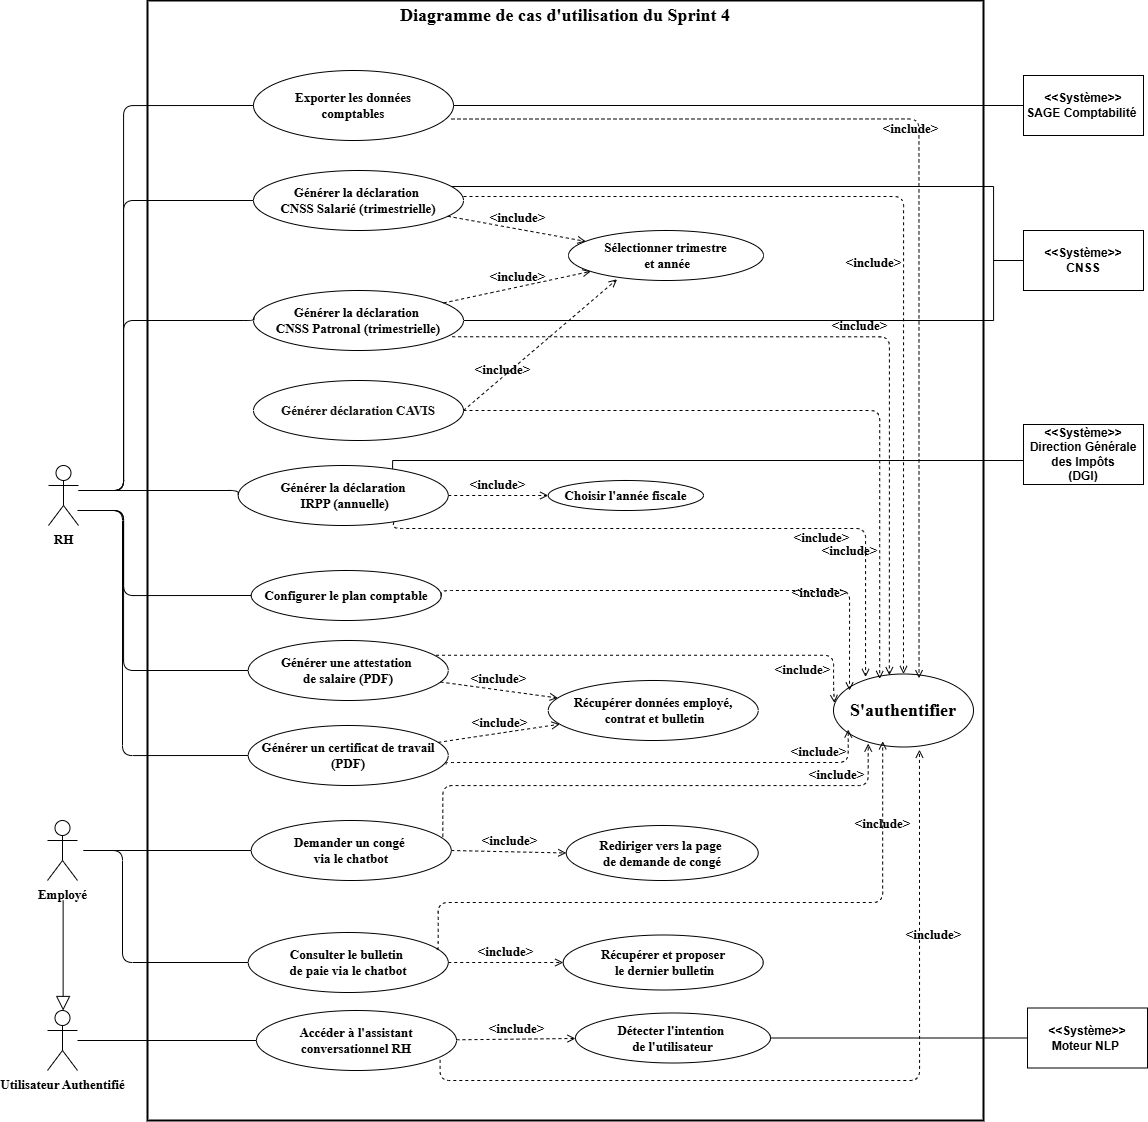
\includegraphics[width=0.95\textwidth]{use-case-sp4.png}
    \caption{Diagramme de cas d'utilisation du Sprint 4}
    \label{fig:use-case-sp4}
\end{figure}

% CORRECTION : Description UC enrichie avec relations UML et responsabilités par rôle précis
Le diagramme de cas d'utilisation du Sprint~4 (Figure~\ref{fig:use-case-sp4})
organise les fonctionnalités en quatre packages distincts, chacun
gouverné par des contraintes d'accès précises.

\textbf{Relations UML~:} Le cas d'utilisation «~Configurer le plan
comptable~» est en relation \texttt{<<include>>} avec
«~Exporter SAGE~», car l'export ne peut produire des écritures
cohérentes que si le plan est configuré. Les quatre actions de
génération de déclarations partagent une précondition commune
(\texttt{<<include>>} «~S'authentifier~» et «~Vérifier périodes
clôturées~»).

\textbf{Responsabilités par acteur~:}

\begin{itemize}[label=\textbullet, leftmargin=0.6cm]
    \item \textbf{Admin / RH Comptable~:}
          Configurer et exporter le plan comptable (CRUD +
          export SAGE). Générer les quatre déclarations
          réglementaires (CNSS salarié/patronal, CAVIS, IRPP).
          Produire les documents officiels (attestations de salaire,
          certificats de travail). Interroger les données RH
          de la société via l'intention \texttt{ADMIN\_SQL}
          du chatbot (effectif, masse salariale, statistiques).

    \item \textbf{Employé~:}
          Accéder au chatbot pour consulter ses données personnelles
          (\texttt{PERSONAL\_SQL}~: salaire, solde de congés,
          ancienneté, poste), initier une demande de congé
          (redirection) et poser des questions réglementaires
          (\texttt{LEGAL\_RAG}~: CNSS, IRPP, code du travail).

    \item \textbf{Utilisateur (tous rôles)~:}
          Accéder aux réponses conversationnelles générales
          (\texttt{GENERAL}~: salutations, questions RH génériques).
\end{itemize}

% -----------------------------------------------------------
\subsection{Description textuelle des cas d'utilisation}
% -----------------------------------------------------------

Les descriptions textuelles suivantes formalisent les préconditions,
scénarios nominaux et alternatifs des cas d'utilisation les plus
critiques du Sprint 4. Elles constituent la référence contractuelle
de validation avec le Product Owner.

% -----------------------------------------------------------
\subsubsection{Cas d'utilisation : Générer les déclarations de conformité réglementaire}
% -----------------------------------------------------------

Le tableau~\ref{tab:cu-conformite} présente la description textuelle
détaillée du cas d'utilisation « Générer les déclarations de conformité
réglementaire ».
\mbox{}\\

\begin{xltabular}{\textwidth}{|l|X|}
\caption{Description textuelle du cas d'utilisation Générer les déclarations de conformité}
\label{tab:cu-conformite} \\
\hline
\rowcolor[gray]{0.9} \textbf{Élément} & \textbf{Description} \\ \hline
\endfirsthead
\hline
\endlastfoot
\textbf{Titre} & Générer les déclarations de conformité réglementaire (CNSS / CAVIS / IRPP) \\ \hline
\textbf{Acteur principal} & RH \\ \hline
\textbf{Préconditions} & Des périodes de paie clôturées (\texttt{LOCKED}) existent pour la période concernée. Les paramètres réglementaires (taux CNSS, CAVIS, barèmes IRPP) sont configurés. \\ \hline
\textbf{Postconditions} & Un fichier déclaratif (CSV ou PDF) est généré et mis à disposition du RH pour téléchargement. \\ \hline
\textbf{Scénario principal} &
\begin{enumerate}[nosep, leftmargin=*]
    \item Le RH accède à l'onglet « Conformité » de la plateforme.
    \item Il sélectionne le type de déclaration souhaitée (CNSS Salarié, CNSS Patronal, CAVIS ou IRPP).
    \item Pour les déclarations trimestrielles, il sélectionne le trimestre et l'année cibles.
    \item Pour la déclaration IRPP, il sélectionne l'exercice fiscal annuel.
    \item Le système agrège les montants correspondants depuis les bulletins clôturés.
    \item Il génère le fichier déclaratif au format réglementaire.
    \item Le fichier est proposé en téléchargement au RH.
\end{enumerate} \\ \hline
\textbf{Scénarios alternatifs}
& \textbf{A1 : Aucune période clôturée} $\rightarrow$ Le système affiche un message indiquant l'absence de données et bloque la génération. \\ \cline{2-2}
& \textbf{A2 : Paramètres réglementaires manquants} $\rightarrow$ Le système lève une erreur bloquante invitant le Super Admin à configurer les taux. \\
\end{xltabular}

% -----------------------------------------------------------
\subsubsection{Cas d'utilisation : Interagir avec l'assistant conversationnel RH}
% -----------------------------------------------------------

Le tableau~\ref{tab:cu-chatbot} présente la description textuelle
détaillée du cas d'utilisation « Interagir avec l'assistant conversationnel RH ».
\mbox{}\\

\begin{xltabular}{\textwidth}{|l|X|}
\caption{Description textuelle du cas d'utilisation Interagir avec le chatbot RH}
\label{tab:cu-chatbot} \\
\hline
\rowcolor[gray]{0.9} \textbf{Élément} & \textbf{Description} \\ \hline
\endfirsthead
\hline
\endlastfoot
\textbf{Titre} & Interagir avec l'assistant conversationnel RH (PaieBot) \\ \hline
\textbf{Acteurs principaux} & Employé --- RH --- Admin \\ \hline
\textbf{Préconditions} & L'utilisateur est authentifié sur la plateforme PaieZone. \\ \hline
\textbf{Postconditions} & L'utilisateur obtient une réponse à sa question RH, est redirigé vers la fonctionnalité adéquate, ou reçoit des statistiques formatées. \\ \hline
\textbf{Scénario principal} &
    \begin{enumerate}[nosep, leftmargin=*]
        \item L'utilisateur clique sur le composant chatbot flottant visible après connexion.
        \item Il saisit sa question en langage naturel.
        \item Le système détecte l'intention parmi quatre catégories~: \texttt{PERSONAL\_SQL}, \texttt{ADMIN\_SQL}, \texttt{LEGAL\_RAG}, \texttt{GENERAL}.
        \item \textbf{Intention \texttt{PERSONAL\_SQL}} : Le pipeline génère une requête SQL sécurisée, l'exécute dans le schéma dédié et retourne le résultat formaté.
        \item \textbf{Intention \texttt{ADMIN\_SQL}} (Admin/RH uniquement) : Même pipeline avec droits élargis pour les statistiques de l'entreprise.
        \item \textbf{Intention \texttt{LEGAL\_RAG}} : Le pipeline RAG recherche dans \texttt{KnowledgeDocument} et génère une réponse contextualisée.
        \item \textbf{Intention \texttt{GENERAL}} : Réponse directe par phi3 en mode conversationnel.
    \end{enumerate} \\ \hline
\textbf{Scénarios alternatifs}
& \textbf{A1 : Intention non reconnue} $\rightarrow$ Le chatbot informe l'utilisateur et propose des exemples de questions reconnues. \\ \cline{2-2}
& \textbf{A2 : Tentative d'accès aux données d'un collègue} $\rightarrow$ Le système refuse avec message de confidentialité, aucune donnée exposée. \\ \cline{2-2}
& \textbf{A3 : SQL dangereux détecté} $\rightarrow$ La requête est rejetée par le validateur de sécurité. \\
\end{xltabular}

% ============================================================
\section{Conception du quatrième Sprint}
\label{sec:s4-conception}
% ============================================================

La conception technique du Sprint 4 traduit les besoins métiers en
modèles structurants guidant le développement. Cette section s'articule
autour de deux axes complémentaires~: le diagramme de classes, qui
modélise l'architecture statique des nouvelles entités, et les
diagrammes de séquence, qui illustrent les interactions dynamiques
entre les composants du système.

% -----------------------------------------------------------
\subsection{Diagramme de classes}
\label{sec:s4-classes}
% -----------------------------------------------------------

Le diagramme de classes du Sprint 4 complète le modèle établi lors du
Sprint 3 en introduisant les entités nécessaires à la comptabilité, à
la conformité, aux documents RH et à l'assistant conversationnel.
Il définit la structure des données ainsi que les relations qui les
unissent avec les entités existantes (\texttt{PayrollPeriod},
\texttt{PaySlip}, \texttt{Employee}, \texttt{Contract}).

La figure~\ref{fig:classes-sprint4} présente le diagramme de classes
du Sprint 4, illustrant l'extension finale du modèle de données de
PaieZone.

\newpage
\begin{figure}[H]
    \vspace*{-0.18cm}
    \centering
    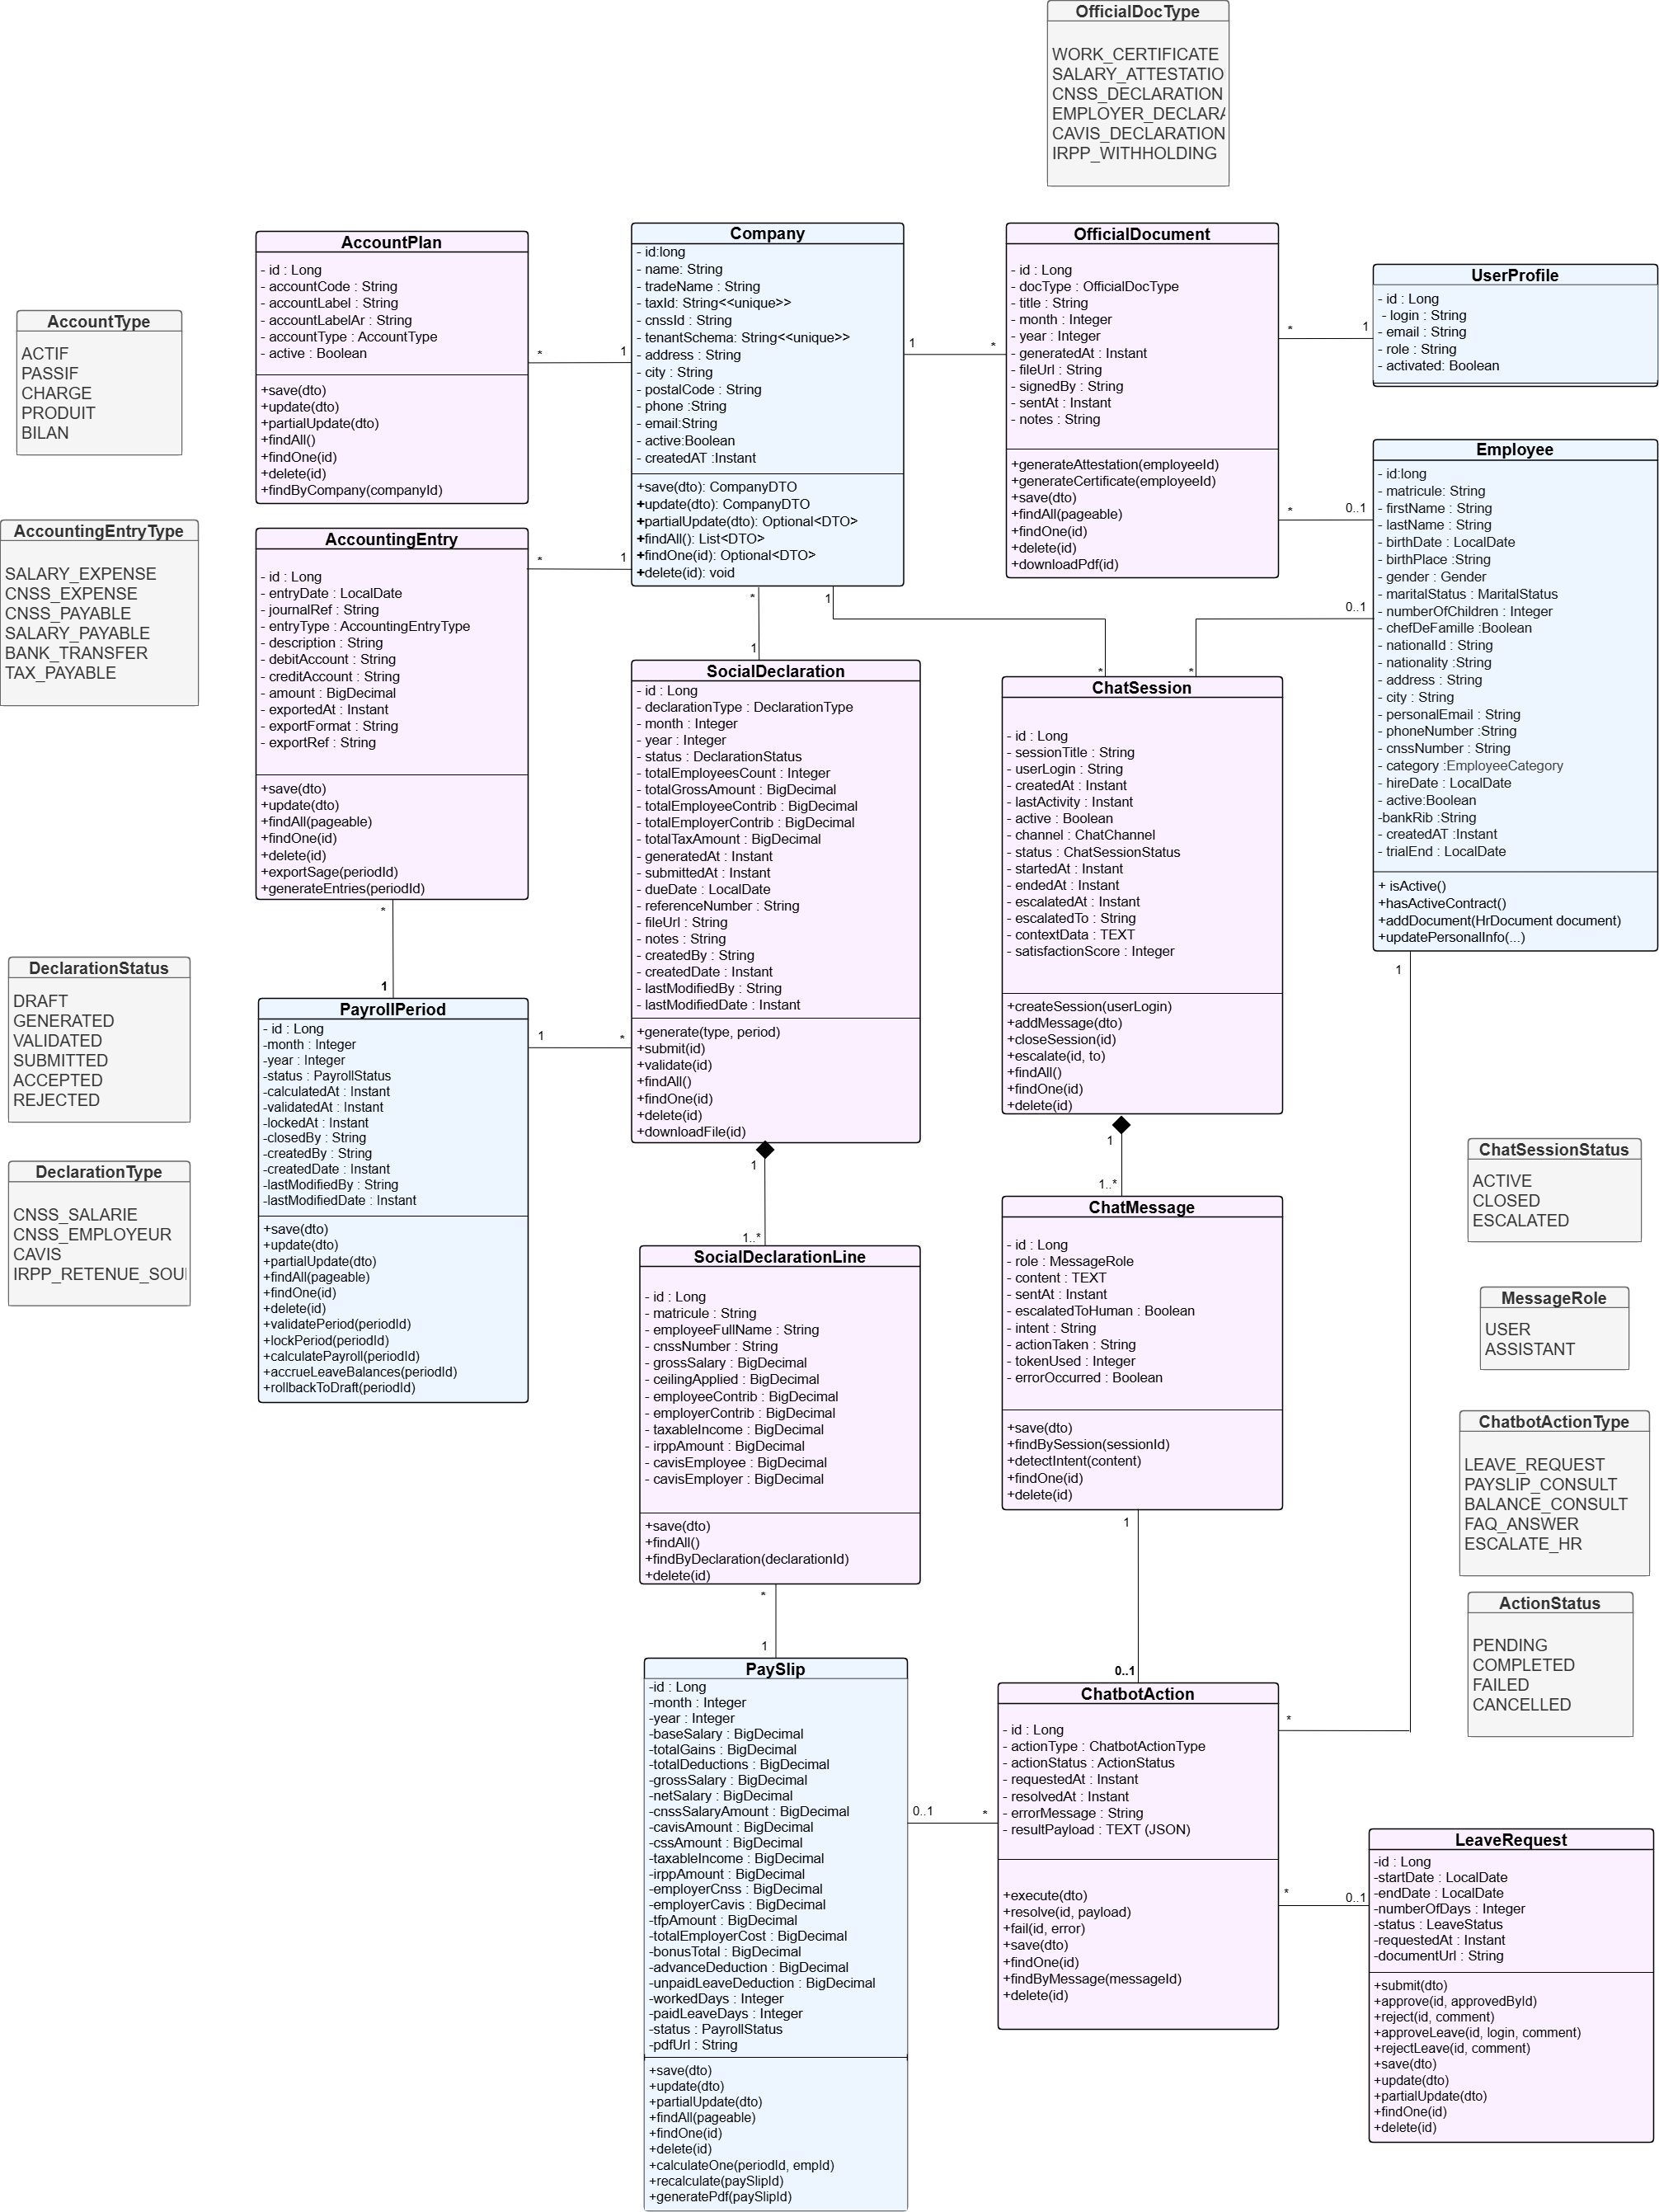
\includegraphics[width=0.95\textwidth]{classes-sprint4.png}
    \caption{Diagramme de classes du Sprint 4}
    \label{fig:classes-sprint4}
\end{figure}

% CORRECTION : Noms corrigés (PayrollPeriod, SocialDeclaration) + entités manquantes ajoutées
% (AccountingEntry, SocialDeclarationLine, ChatSession, ChatMessage, KnowledgeDocument)
Les entités principales introduites dans ce sprint sont les
suivantes~:

\begin{itemize}[label=\textbullet, leftmargin=0.6cm]

    \item \textbf{\texttt{AccountPlan}}~: modélise le plan comptable
          de la société. Chaque entrée associe un code de compte
          (\texttt{accountCode}), un libellé (\texttt{label}), un type
          (\texttt{accountType}) et optionnellement une rubrique de
          paie (\texttt{Rubrique}), permettant la génération de
          l'export comptable SAGE.

    \item \textbf{\texttt{AccountingEntry}}~: représente une écriture
          comptable individuelle générée depuis un bulletin de paie.
          Elle lie un \texttt{AccountPlan}, un \texttt{PaySlip} et
          enregistre le montant, le sens (débit/crédit) et le type
          de l'écriture (\texttt{AccountingEntryType}).

    \item \textbf{\texttt{SocialDeclaration}}~: conserve les données
          agrégées de chaque déclaration réglementaire générée
          (type~: CNSS\_SALARY, CNSS\_EMPLOYER, CAVIS, IRPP~;
          période de référence~; totaux salarié/patronal~; statut~;
          horodatage de génération~; URL du fichier produit).
          Liée à \texttt{Company} et \texttt{PayrollPeriod}.

    \item \textbf{\texttt{SocialDeclarationLine}}~: détail ligne
          par ligne de la déclaration, avec le montant individuel
          par employé, permettant la traçabilité des montants
          déclarés.

    \item \textbf{\texttt{OfficialDocument}}~: stocke les métadonnées
          des documents officiels générés automatiquement
          (attestations de salaire, certificats de travail,
          fichiers de déclaration)~; typé via \texttt{OfficialDocType}
          (WORK\_CERTIFICATE, SALARY\_ATTESTATION,
          CNSS\_DECLARATION, CAVIS\_DECLARATION,
          IRPP\_WITHHOLDING). Liée à \texttt{Employee}.

    \item \textbf{\texttt{ChatSession}}~: session de conversation
          PaieBot identifiée par \texttt{userLogin}. Porte le titre
          de la session (auto-généré depuis le premier message),
          les horodatages de création et de dernière activité,
          et le statut actif/fermé.

    \item \textbf{\texttt{ChatMessage}}~: message unitaire de la
          conversation. Stocke le rôle (\texttt{USER} ou
          \texttt{ASSISTANT}), le contenu, l'intention détectée
          (\texttt{IntentType}~: PERSONAL\_SQL, ADMIN\_SQL,
          LEGAL\_RAG, GENERAL) et un indicateur d'escalade vers
          le RH humain (\texttt{escalatedToHuman}).

    \item \textbf{\texttt{KnowledgeDocument}}~: base documentaire
          du système RAG. Chaque document porte un titre, un
          contenu textuel, une catégorie et des mots-clés indexés
          (\texttt{keywords}) utilisés pour la correspondance lors
          des requêtes \texttt{LEGAL\_RAG}.

\end{itemize}

% -----------------------------------------------------------
\subsection{Diagrammes de séquences}
% -----------------------------------------------------------

Les diagrammes de séquences illustrent la dynamique du système en
détaillant les interactions chronologiques entre les composants pour
les cas d'utilisation les plus critiques.

% -----------------------------------------------------------
\subsubsection{Diagramme de séquence : Générer une déclaration de conformité}
% -----------------------------------------------------------

La figure~\ref{fig:seq-conformite} illustre le flux de génération
d'une déclaration réglementaire (CNSS, CAVIS ou IRPP).

\begin{figure}[H]
    \vspace*{-0.18cm}
    \centering
    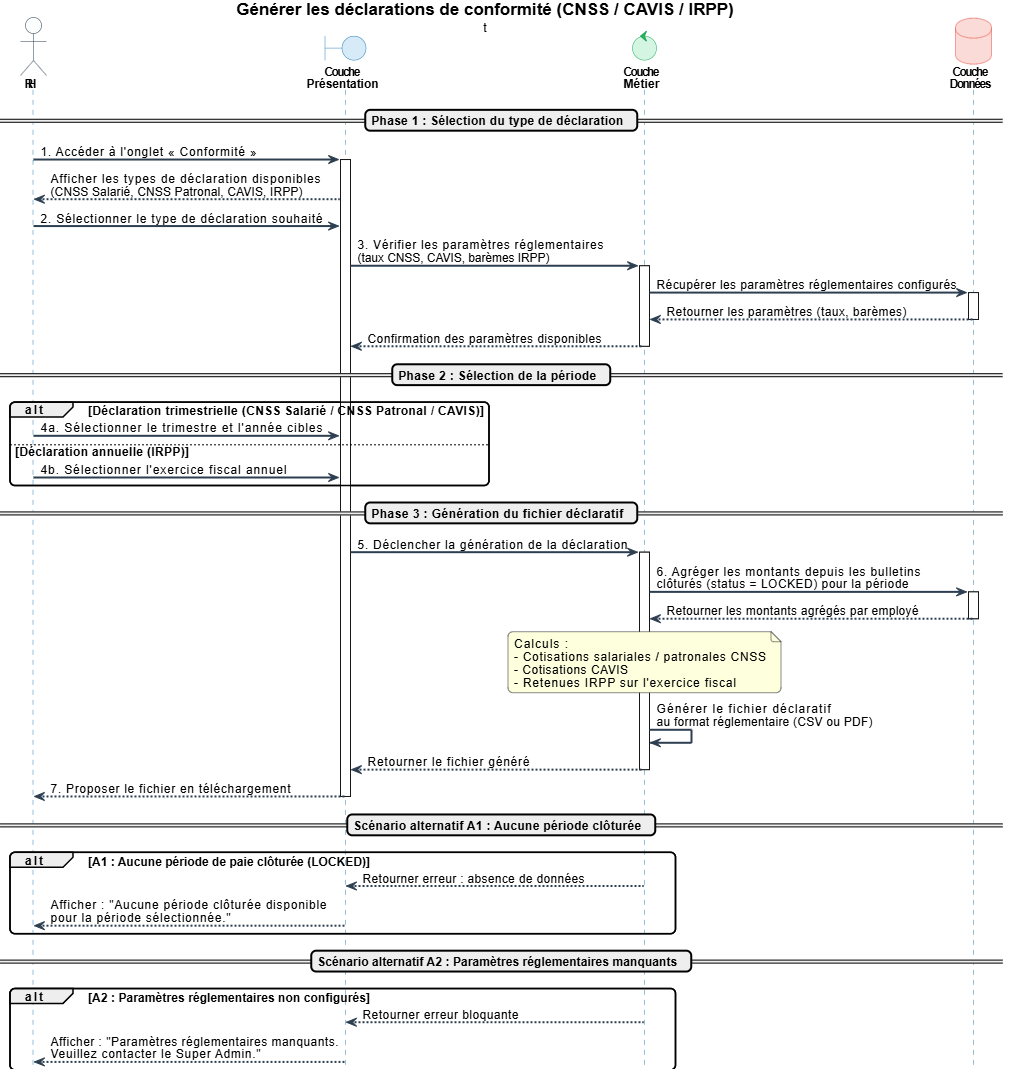
\includegraphics[width=0.85\textwidth]{seq-sp4-uc1.png}
    \caption{Diagramme de séquence --- Générer une déclaration de conformité}
    \label{fig:seq-conformite}
\end{figure}

Ce diagramme illustre l'agrégation automatique des données financières
issues des bulletins clôturés pour produire un fichier déclaratif
conforme aux exigences des organismes tunisiens~\cite{cnss_reg,lf2026}.
Le flux garantit l'intégrité des montants déclarés par rapport aux
données calculées lors du cycle de paie.

% -----------------------------------------------------------
\subsubsection{Diagramme de séquence : Interaction avec le chatbot RH}
% -----------------------------------------------------------

La figure~\ref{fig:seq-chatbot} illustre le flux d'interaction entre
un utilisateur et l'assistant conversationnel RH de PaieZone.

\begin{figure}[H]
    \vspace*{-0.18cm}
    \centering
    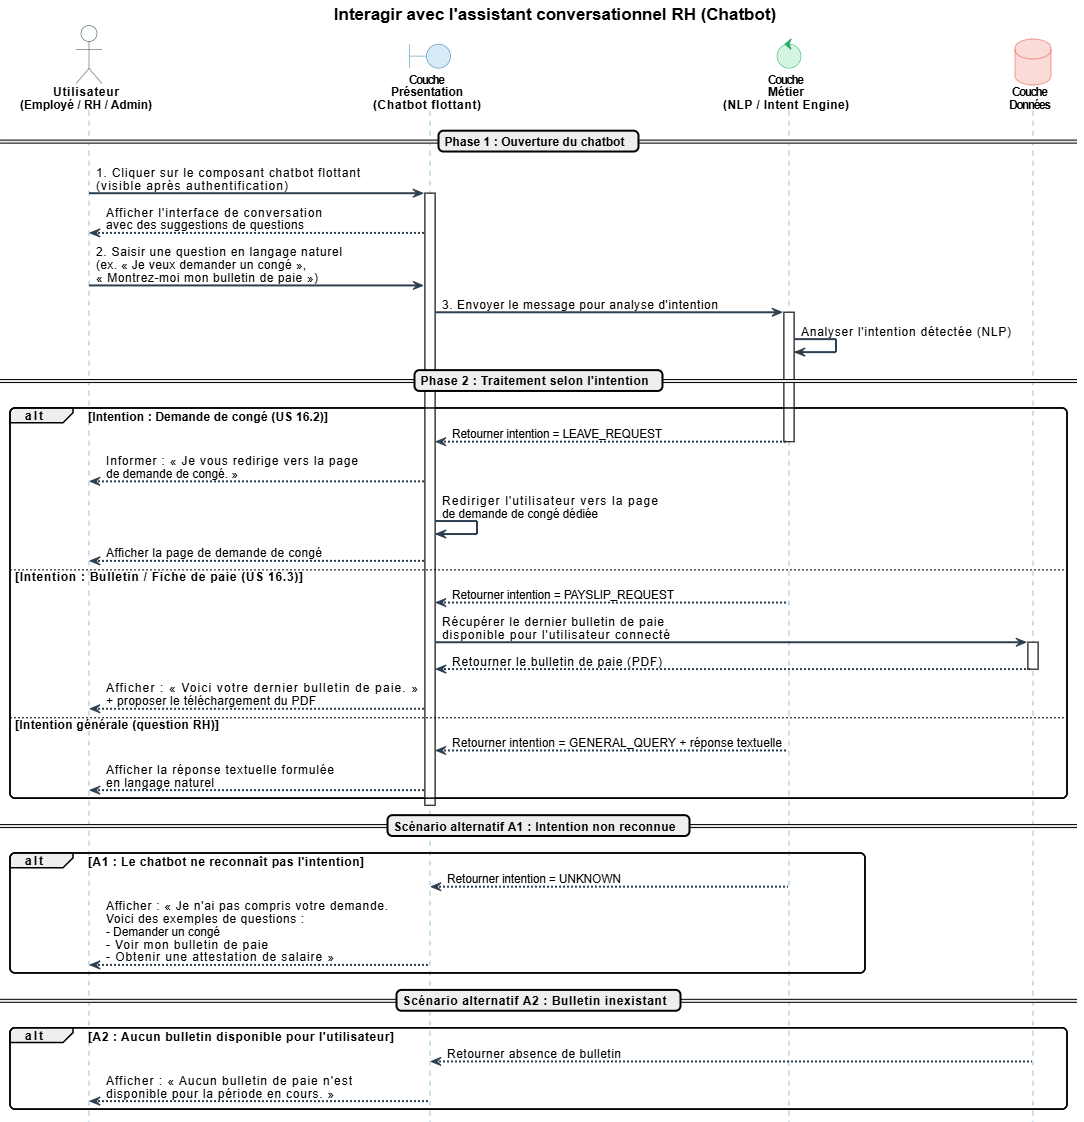
\includegraphics[width=0.80\textwidth]{seq-sp4-uc2.png}
    \caption{Diagramme de séquence --- Interaction avec le chatbot RH}
    \label{fig:seq-chatbot}
\end{figure}
\newpage

% CORRECTION : "détection légère des intentions" remplacé par description technique complète
Ce diagramme modélise le pipeline complet de traitement d'un message
utilisateur par PaieBot, l'assistant conversationnel de PaieZone~RH.

\textbf{Architecture à quatre intentions~:} À réception d'un message,
\texttt{TextToSqlService.detectIntent()} analyse le texte normalisé
et le classe parmi quatre catégories~:

\begin{itemize}[label=\textbullet, leftmargin=0.6cm]
    \item \textbf{\texttt{PERSONAL\_SQL}}~: questions de l'employé sur
          ses propres données (salaire, congés, ancienneté, poste).
          Le pipeline génère une requête SQL via Ollama~phi3
          (température 0,05 --- déterministe), la valide, l'exécute
          dans le schéma PostgreSQL~\cite{postgresql} du tenant, et formate le résultat
          en Markdown.

    \item \textbf{\texttt{ADMIN\_SQL}}~: questions RH/Admin sur les
          données de l'entreprise (effectif, masse salariale,
          répartition). Même pipeline SQL avec droits élargis
          (pas de filtre \texttt{user\_profile\_id}).

    \item \textbf{\texttt{LEGAL\_RAG}}~: questions réglementaires
          (CNSS, IRPP, code du travail, conventions collectives).
          Les documents \texttt{KnowledgeDocument} correspondant
          aux mots-clés de la question sont injectés dans le prompt
          système d'Ollama (RAG~\cite{rag}). La réponse est générée par phi3
          en mode conversationnel (température 0,7).

    \item \textbf{\texttt{GENERAL}}~: salutations et questions
          génériques traitées directement par phi3~\cite{phi3} sans base de
          connaissances.
\end{itemize}

\textbf{Garanties de sécurité~:} Avant tout traitement, le système
vérifie qu'un employé n'essaie pas d'accéder aux données d'un
collègue (protection inter-tenant). Les requêtes SQL générées
sont systématiquement validées (blocage de DROP, DELETE, ALTER,
TRUNCATE, etc.) et exécutées avec \texttt{SET search\_path} pour
l'isolation multi-tenant. Les réponses contenant des hallucinations
caractéristiques de phi3 sont détectées par analyse regex et
remplacées par un message d'erreur générique.

% ============================================================
\section{Étude et réalisation du quatrième sprint}
\label{sec:s4-realisation}
% ============================================================

Cette section présente les réalisations concrètes du Sprint 4, marquant
la finalisation de la plateforme PaieZone. Les travaux ont porté sur
l'implémentation du module comptable, la génération des déclarations
réglementaires, la production automatisée des documents administratifs
RH et le déploiement de l'assistant conversationnel PaieBot.

% ============================================================
\subsection{Gestion comptable et export SAGE}
% ============================================================

\begin{figure}[H]
    \vspace*{-0.18cm}
    \centering
    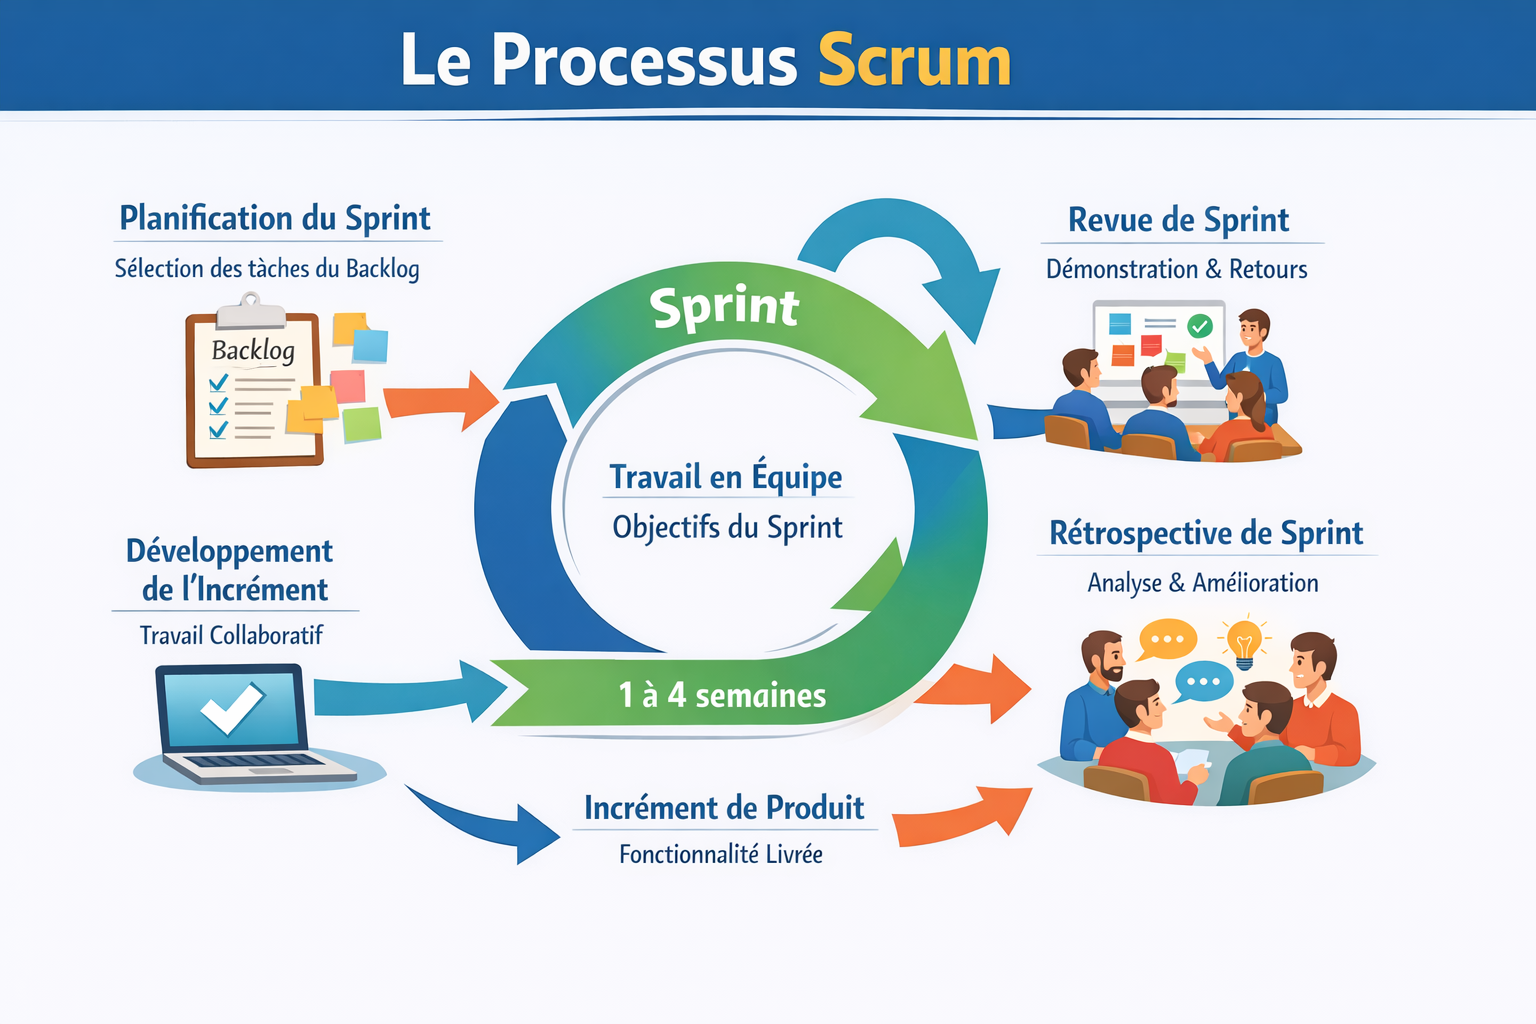
\includegraphics[width=0.70\textwidth]{scrum.png}
    \caption{Interface de gestion du plan comptable et export SAGE}
    \label{fig:ui-comptabilite}
\end{figure}

La figure~\ref{fig:ui-comptabilite} présente l'interface de l'onglet
Comptabilité de PaieZone. Le RH ou l'Administrateur dispose d'un
tableau de gestion du plan comptable offrant un CRUD complet (création,
modification, suppression de comptes). Un bouton « Exporter SAGE (.csv) »
permet de générer à la demande un fichier d'export conforme au format
attendu par les logiciels comptables SAGE, contenant les écritures
issues des bulletins de paie clôturés.

% ============================================================
\subsection{Conformité réglementaire}
% ============================================================

\begin{figure}[H]
    \vspace*{-0.18cm}
    \centering
    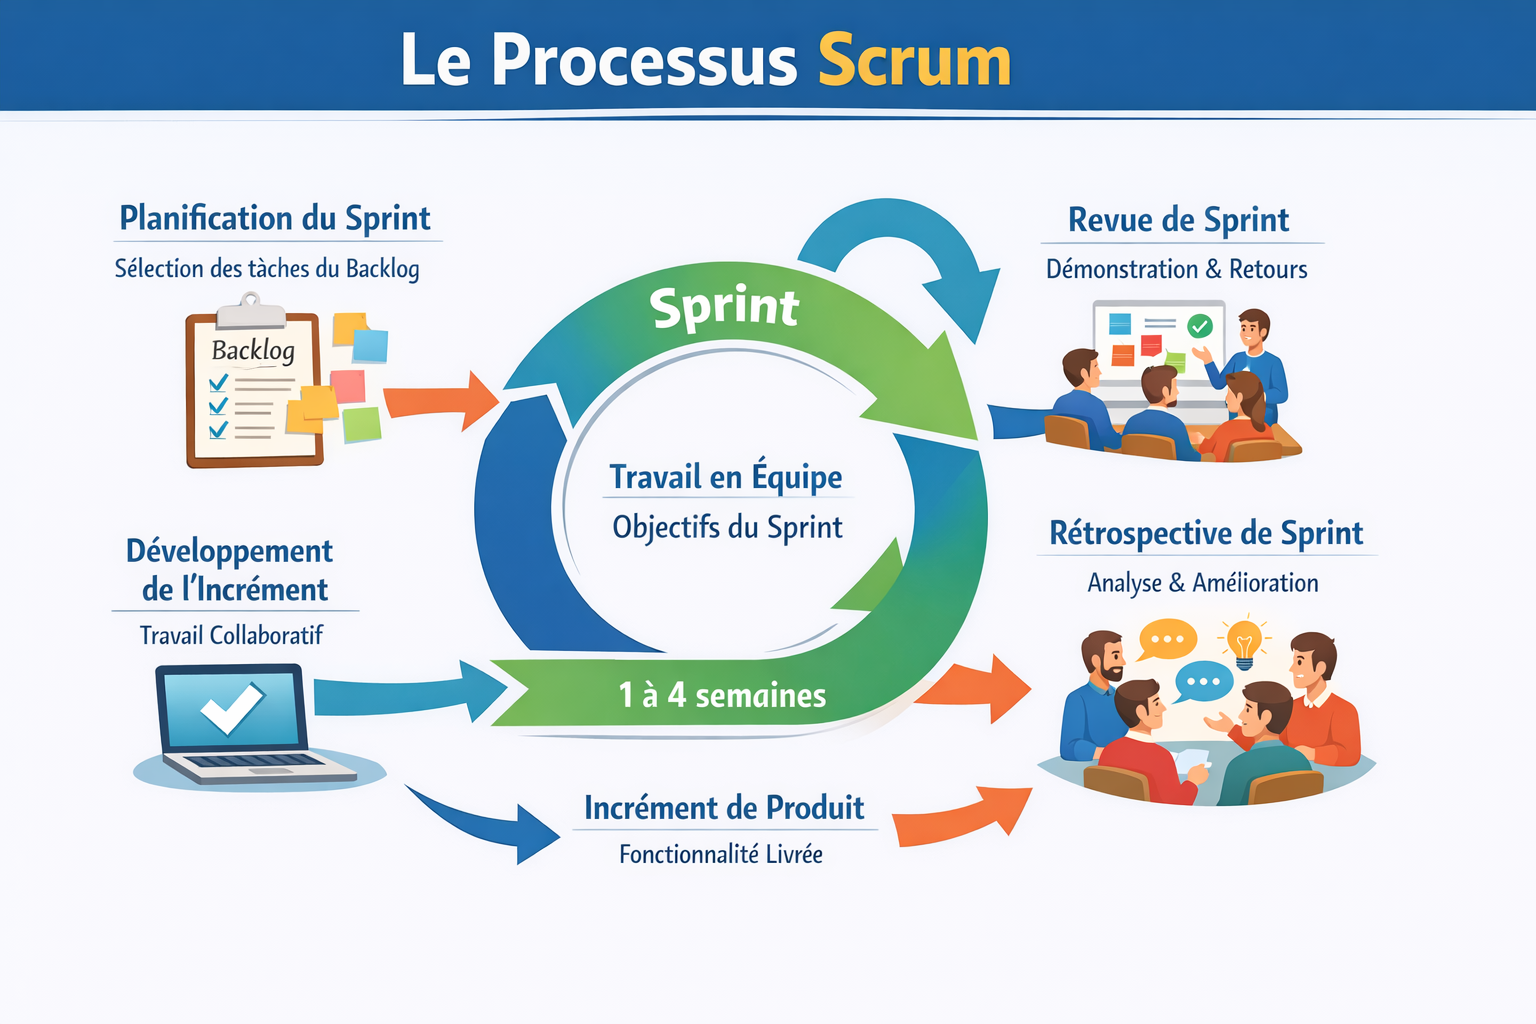
\includegraphics[width=0.70\textwidth]{scrum.png}
    \caption{Interface de l'onglet Conformité --- Déclarations CNSS, CAVIS et IRPP}
    \label{fig:ui-conformite}
\end{figure}

La figure~\ref{fig:ui-conformite} présente le module de conformité
réglementaire. Le RH accède à quatre actions de génération~:
déclaration CNSS salarié, déclaration CNSS patronal, déclaration
CAVIS (toutes trois au pas trimestriel) et déclaration IRPP
(annuelle). Chaque déclenchement agrège automatiquement les montants
depuis les bulletins clôturés de la période sélectionnée et produit
un fichier téléchargeable conforme aux exigences légales
tunisiennes~\cite{loifinance,cnss_reg}.

% ============================================================
\subsection{Documents administratifs RH}
% ============================================================

\begin{figure}[H]
    \vspace*{-0.18cm}
    \centering
    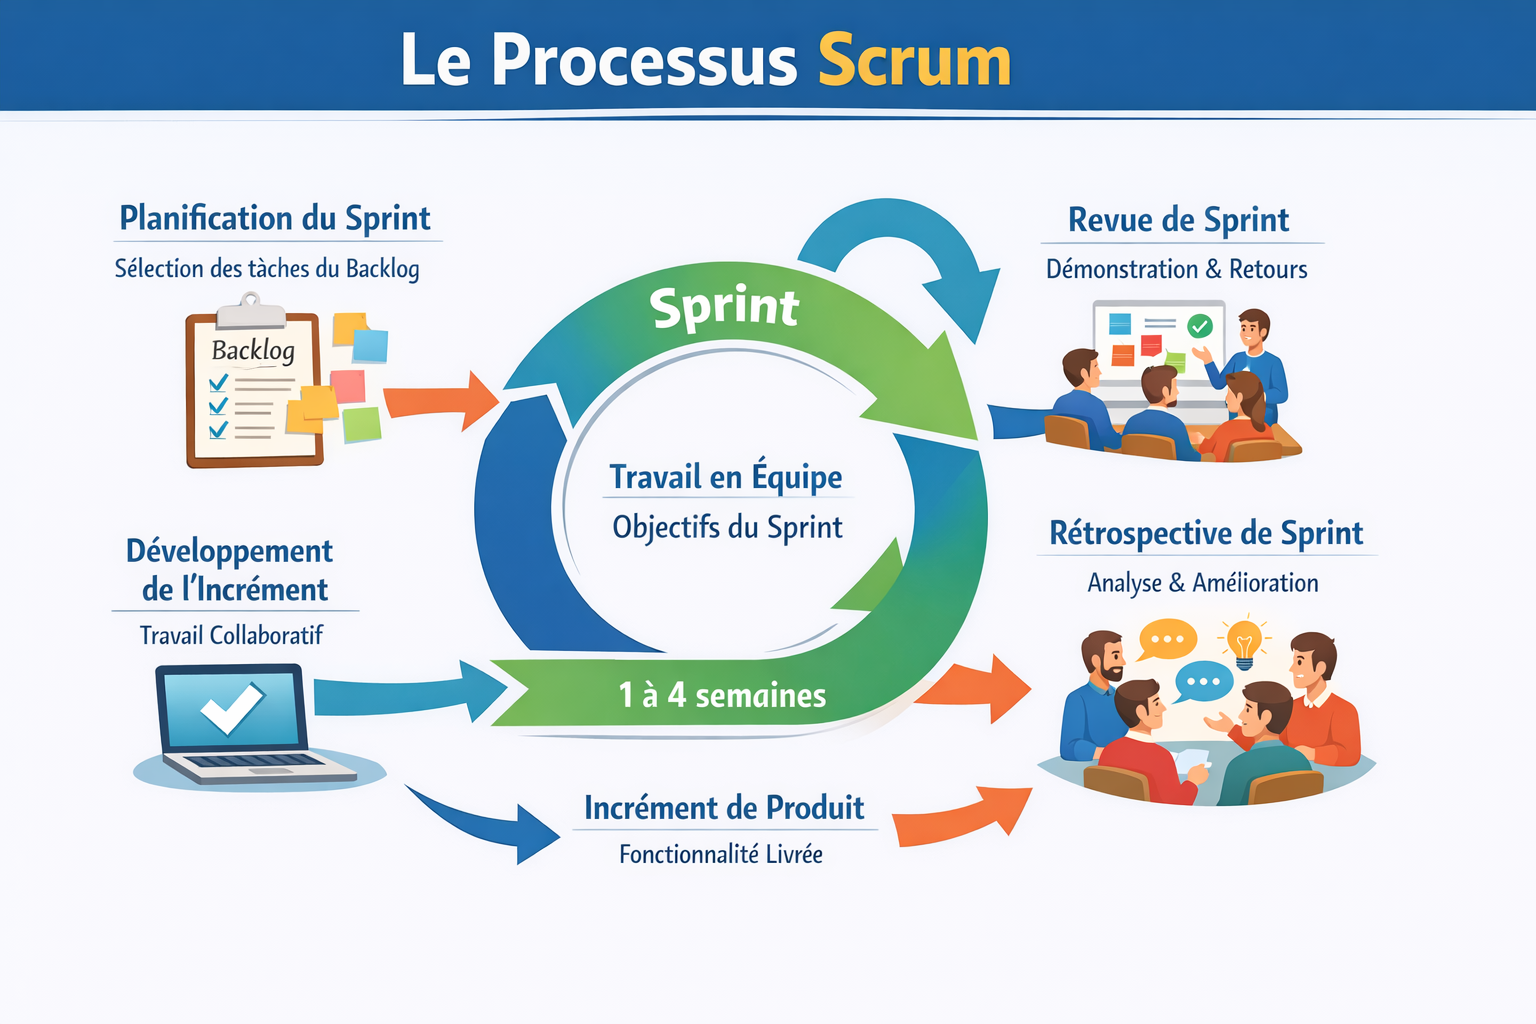
\includegraphics[width=0.70\textwidth]{scrum.png}
    \caption{Génération de l'attestation de salaire et du certificat de travail}
    \label{fig:ui-docs-rh}
\end{figure}

La figure~\ref{fig:ui-docs-rh} illustre la fonctionnalité de génération
des documents administratifs RH accessible depuis la page Employés.
Un clic sur le bouton de téléchargement PDF déclenche la génération
de l'attestation de salaire ou du certificat de travail via le moteur
\textbf{Flying Saucer}~\cite{flyingsaucer} (\texttt{ITextRenderer}),
directement alimentés par les données du dossier employé et de son
dernier bulletin calculé. Les documents respectent les templates
légaux en vigueur et sont disponibles immédiatement en téléchargement.

% ============================================================
\subsection{Assistant conversationnel RH (PaieBot)}
\label{sec:s4-chatbot}
% ============================================================

\begin{figure}[H]
    \vspace*{-0.18cm}
    \centering
    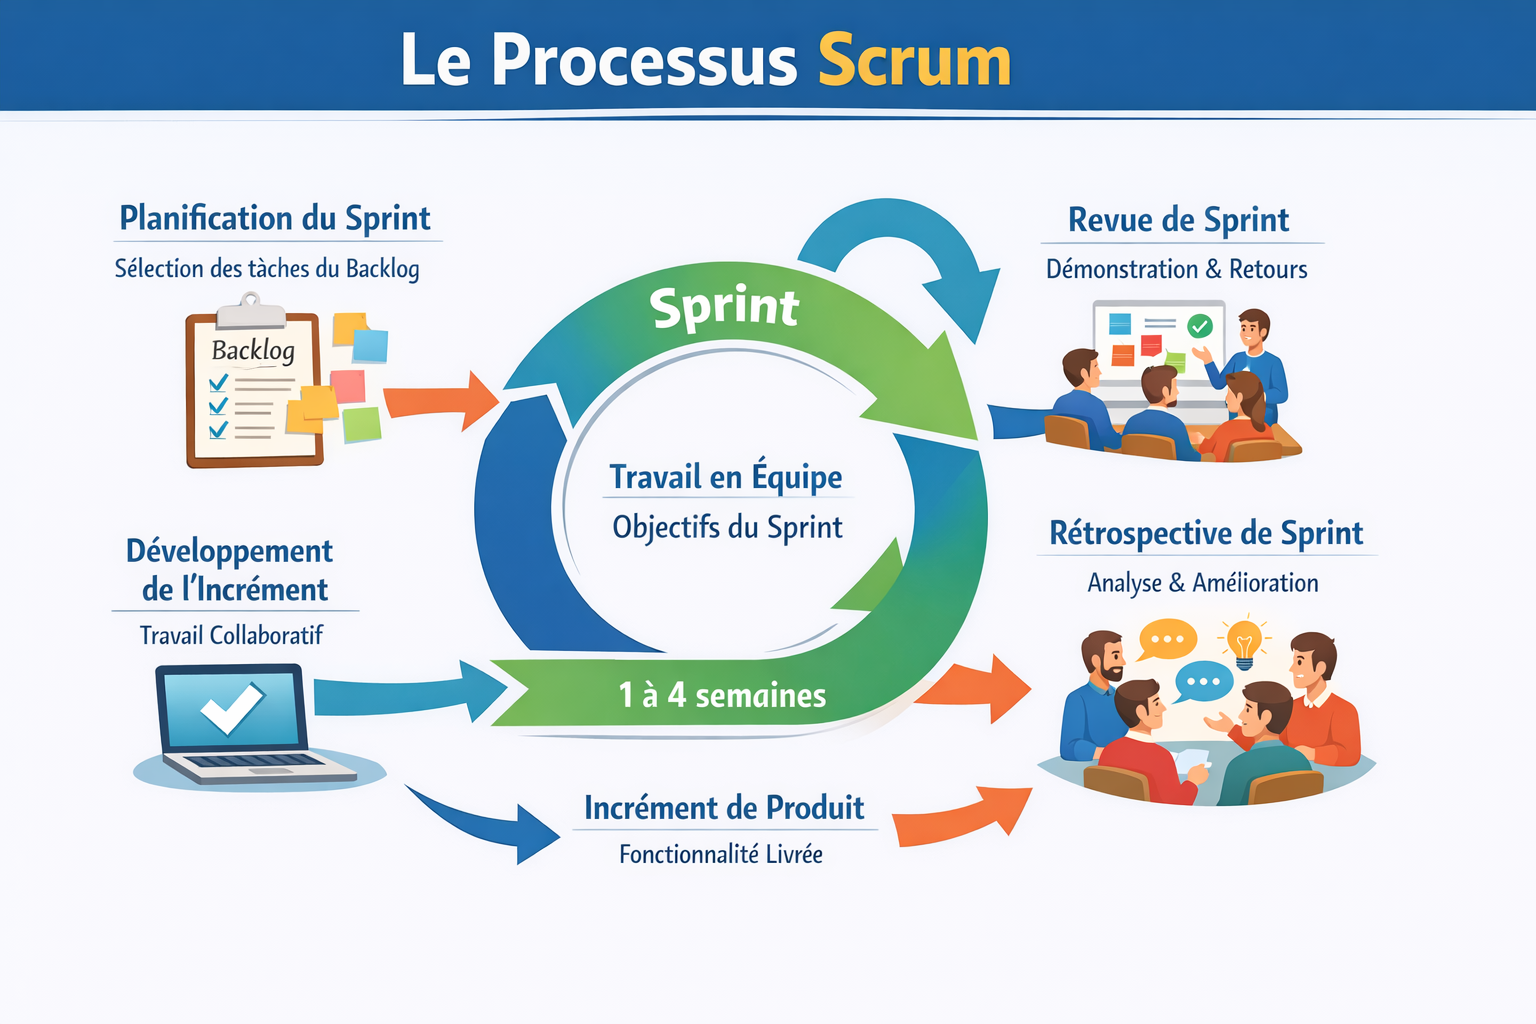
\includegraphics[width=0.70\textwidth]{scrum.png}
    \caption{Composant PaieBot --- Assistant conversationnel RH flottant}
    \label{fig:ui-chatbot}
\end{figure}

% CORRECTION : Description complète des 4 intentions + mécanismes de sécurité
La figure~\ref{fig:ui-chatbot} présente le composant chatbot flottant
PaieBot de PaieZone~RH, visible par tous les utilisateurs après
authentification. L'assistant traite quatre catégories de requêtes~:

\begin{itemize}[label=\textbullet, leftmargin=0.6cm]
    \item \textbf{Données personnelles (\texttt{PERSONAL\_SQL})~:}
          L'employé peut interroger ses propres informations en langage
          naturel («~Quel est mon salaire net~?~», «~Combien de jours de
          congé me restent~?~», «~Quel est mon poste~?~»). Le système
          génère une requête SQL sécurisée, l'exécute dans le schéma
          dédié et retourne le résultat formaté.

    \item \textbf{Statistiques RH (\texttt{ADMIN\_SQL})~:}
          Pour les rôles Admin et RH uniquement, PaieBot peut répondre
          à des questions agrégées («~Combien d'employés actifs~?~»,
          «~Quelle est la masse salariale~?~», «~Effectif par
          département~?~»).

    \item \textbf{Réglementation (\texttt{LEGAL\_RAG})~:}
          Les questions sur le code du travail tunisien, les taux CNSS
          et IRPP, les conventions collectives ou les congés légaux
          sont traitées par le pipeline RAG~\cite{rag}~: recherche dans la base
          documentaire (\texttt{KnowledgeDocument}) et génération d'une
          réponse contextualisée par le modèle phi3~\cite{phi3}.

    \item \textbf{Général (\texttt{GENERAL})~:}
          Salutations et questions courtes traitées directement par
          phi3~\cite{phi3} en mode conversationnel.
\end{itemize}

Les mécanismes de sécurité implémentés garantissent~: l'isolation
des données par tenant, le blocage des requêtes inter-employés,
la détection et la suppression des hallucinations du modèle,
et l'escalade automatique vers le service RH pour les situations
d'urgence détectées.

% ============================================================
\section{Tests et Validation}
\label{sec:s4-tests}
% ============================================================

La phase de tests et de validation du Sprint 4 vise à garantir la
conformité des fichiers déclaratifs produits et la fiabilité de
l'assistant conversationnel. Trois niveaux de tests ont été mis en
œuvre de manière complémentaire.

% -----------------------------------------------------------
\subsection{Plan de tests}
% -----------------------------------------------------------

\begin{itemize}[label=\textbullet, leftmargin=0.6cm]
    \item \textbf{Tests unitaires (JUnit~5, Mockito)} : Validation des
    services de génération --- notamment les algorithmes d'agrégation
    des montants CNSS, CAVIS et IRPP, et la cohérence des écritures
    comptables produites.
    \item \textbf{Tests d'intégration} : Validation des flux complets ---
    génération des déclarations sur des périodes clôturées réelles,
    export SAGE et vérification des montants par rapprochement avec
    les bulletins sources.
    \item \textbf{Tests fonctionnels (interface Angular~\cite{angular})} : Vérification
    du comportement des formulaires, de la conformité des PDF générés,
    et de la robustesse du chatbot face aux quatre intentions et aux
    cas limites de sécurité.
\end{itemize}

\vspace{0.4cm}
% CORRECTION : Tableau renommé 6.6 (éviter duplication avec Table 6.2 du Backlog)
% + Tests chatbot enrichis : PERSONAL_SQL, LEGAL_RAG, sécurité inter-tenant, SQL dangereux
Le Tableau~\ref{tab:tests-sprint4-recap} synthétise les cas de test principaux
réalisés pour ce sprint.

\renewcommand{\arraystretch}{1.3}
\begin{longtable}{|c|p{7.5cm}|p{4.5cm}|c|}
\caption{Récapitulatif des cas de test du Sprint~4}
\label{tab:tests-sprint4-recap} \\
\hline
\textbf{ID Test} &
\textbf{Description du cas de test} &
\textbf{Résultat attendu} &
\textbf{Statut} \\
\hline
\endfirsthead
\hline
\textbf{ID Test} &
\textbf{Description du cas de test} &
\textbf{Résultat attendu} &
\textbf{Statut} \\
\hline
\endhead
\hline
\endfoot
\hline
\endlastfoot

T-13.1 & CRUD complet du plan comptable & Opérations sans erreur, données persistées & \textcolor{green!60!black}{\textbf{OK}} \\ \hline
T-13.2 & Export SAGE sur une période clôturée & Fichier CSV conforme au format SAGE, téléchargeable & \textcolor{green!60!black}{\textbf{OK}} \\ \hline
T-14.1 & Génération CNSS salarié pour un trimestre avec 5 employés & Montants cohérents avec les bulletins calculés & \textcolor{green!60!black}{\textbf{OK}} \\ \hline
T-14.2 & Génération CNSS patronal trimestrielle & Montants patronaux conformes aux taux configurés & \textcolor{green!60!black}{\textbf{OK}} \\ \hline
T-14.3 & Génération CAVIS trimestrielle & Fichier CAVIS conforme aux exigences légales & \textcolor{green!60!black}{\textbf{OK}} \\ \hline
T-14.4 & Génération IRPP annuelle sur un exercice complet & État récapitulatif IRPP conforme aux exigences DGI & \textcolor{green!60!black}{\textbf{OK}} \\ \hline
T-14.5 & Génération d'une déclaration sans période clôturée & Erreur bloquante, aucun fichier généré & \textcolor{green!60!black}{\textbf{OK}} \\ \hline
T-15.1 & Génération de l'attestation de salaire PDF & PDF conforme au template avec données correctes & \textcolor{green!60!black}{\textbf{OK}} \\ \hline
T-15.2 & Génération du certificat de travail PDF & PDF avec données contractuelles exactes & \textcolor{green!60!black}{\textbf{OK}} \\ \hline
T-16.1 & Affichage du composant chatbot après authentification (tous rôles) & Composant flottant visible pour tous les rôles & \textcolor{green!60!black}{\textbf{OK}} \\ \hline
T-16.2 & Intention \texttt{PERSONAL\_SQL}~: «~Quel est mon salaire net~?~» & Résultat SQL formaté avec le salaire net de l'employé connecté & \textcolor{green!60!black}{\textbf{OK}} \\ \hline
T-16.3 & Intention \texttt{ADMIN\_SQL} (rôle RH)~: «~Effectif par département~» & Tableau Markdown avec les données de l'entreprise du tenant & \textcolor{green!60!black}{\textbf{OK}} \\ \hline
T-16.4 & Intention \texttt{LEGAL\_RAG}~: question sur le taux CNSS & Réponse basée sur \texttt{KnowledgeDocument}, conforme à la LF 2026 & \textcolor{green!60!black}{\textbf{OK}} \\ \hline
T-16.5 & Tentative d'accès aux données d'un autre employé & Refus avec message de confidentialité, aucune donnée exposée & \textcolor{green!60!black}{\textbf{OK}} \\ \hline
T-16.6 & Intention «~congé~» --- redirection & Redirection vers la page \texttt{/paiezone/emp-leaves} & \textcolor{green!60!black}{\textbf{OK}} \\ \hline
T-16.7 & SQL dangereux injecté dans la question (\texttt{DROP TABLE}) & Requête rejetée par le validateur de sécurité, message d'erreur & \textcolor{green!60!black}{\textbf{OK}} \\ \hline

\end{longtable}
\renewcommand{\arraystretch}{1.0}

% -----------------------------------------------------------
\subsection{Tests automatisés}
% -----------------------------------------------------------

Le Sprint~4 couvre les fonctionnalités les plus avancées de \pz{}~:
l'assistant conversationnel IA et les conventions sectorielles. Deux
risques critiques ont motivé une couverture de tests approfondie~:
la fuite d'informations cross-tenant via le chatbot et les
hallucinations du modèle phi3.

\paragraph{ChatbotServiceTest --- 13 cas de test (JUnit~5 + Mockito)}

\renewcommand{\arraystretch}{1.2}
\begin{small}
\begin{longtable}{|c|p{5.5cm}|p{3.8cm}|c|}
\hline
\rowcolor[gray]{0.9}
\textbf{ID} & \textbf{Scénario} & \textbf{Résultat attendu} & \textbf{Statut} \\ \hline
\endfirsthead \hline
\rowcolor[gray]{0.9}
\textbf{ID} & \textbf{Scénario} & \textbf{Résultat attendu} & \textbf{Statut} \\ \hline
\endhead \hline \endfoot \hline
\caption{Tests automatisés --- ChatbotServiceTest}\label{tab:auto-chatbot}\endlastfoot
TA-S4-01 & Création de session avec titre
    & DTO retourné, sauvegarde en base & \textcolor{green!60!black}{\textbf{OK}} \\ \hline
TA-S4-02 & Création de session sans titre
    & Titre = «~Nouvelle conversation~» & \textcolor{green!60!black}{\textbf{OK}} \\ \hline
TA-S4-03 & Accès à une session inexistante
    & HTTP 404 & \textcolor{green!60!black}{\textbf{OK}} \\ \hline
TA-S4-04 & Accès à la session d'un autre utilisateur
    & HTTP 404 (sécurité par obscurité) & \textcolor{green!60!black}{\textbf{OK}} \\ \hline
TA-S4-05 & Employé demande le salaire d'un collègue
    & Refus immédiat, Ollama non appelé & \textcolor{green!60!black}{\textbf{OK}} \\ \hline
TA-S4-06 & Admin envoie la même requête cross-tenant
    & Accès accordé, réponse retournée & \textcolor{green!60!black}{\textbf{OK}} \\ \hline
TA-S4-07 & Réponse phi3 contenant un email inventé
    & Email remplacé par message sûr & \textcolor{green!60!black}{\textbf{OK}} \\ \hline
TA-S4-08 & Réponse phi3 avec «~I'm sorry, but I cannot~»
    & Réponse remplacée & \textcolor{green!60!black}{\textbf{OK}} \\ \hline
TA-S4-09 & Réponse légitime phi3
    & Réponse conservée sans modification & \textcolor{green!60!black}{\textbf{OK}} \\ \hline
TA-S4-10 & Intention \texttt{ADMIN\_SQL} par un employé
    & Reclassifiée en \texttt{LEGAL\_RAG} & \textcolor{green!60!black}{\textbf{OK}} \\ \hline
TA-S4-11 & Intention \texttt{ADMIN\_SQL} par un RH Comptable
    & SQL exécuté, résultat retourné & \textcolor{green!60!black}{\textbf{OK}} \\ \hline
TA-S4-12 & Réponse contenant \texttt{[ESCALADE\_RH]}
    & \texttt{escalatedToHuman = true} & \textcolor{green!60!black}{\textbf{OK}} \\ \hline
TA-S4-13 & Tests E2E Cypress~: ouverture PaieBot, envoi message
    & Bulle utilisateur visible, réponse bot reçue & \textcolor{green!60!black}{\textbf{OK}} \\ \hline
\end{longtable}
\end{small}
\renewcommand{\arraystretch}{1.0}

\paragraph{Bug détecté et corrigé lors des tests}
L'écriture du test TA-S4-07 a révélé une anomalie~: le Signal Angular
\texttt{companiesLoaded} du \texttt{DataService} était positionné à
\texttt{true} même en cas d'erreur HTTP~500 sur l'endpoint
\texttt{/api/companies}, rendant le dashboard SaaS silencieusement vide.
Un nouveau Signal \texttt{companiesError} a été ajouté au
\texttt{DataService} et un mécanisme de retry a été intégré dans le
\texttt{SaasDashboardComponent}, garantissant que les données s'affichent
correctement après une erreur réseau transitoire.

\textbf{Résultat global Sprint~4~:} 13/13 tests automatisés passés
(\textcolor{green!60!black}{\textbf{OK}}), couverture estimée à
\textbf{72\,\%} pour \texttt{ChatbotService}.

% ============================================================
\section{Rituels Agiles et Clôture du Sprint}
\label{sec:s4-rituels}
% ============================================================

Conformément à la méthodologie Scrum~\cite{scrumguide} adoptée par l'équipe PaieZone,
le Sprint 4 s'est clôturé par la tenue des deux rituels essentiels~:
la Sprint Review et la Sprint Retrospective. Ces cérémonies assurent
la transparence du travail accompli et l'amélioration continue des
pratiques d'équipe.

% ============================================================
\subsection{Revue du Sprint (Sprint Review)}
% ============================================================

La Sprint Review a réuni l'équipe de développement, le Product Owner
et les parties prenantes. Les User Stories du sprint ont été présentées
et démontrées en conditions réelles à travers l'interface Angular~\cite{angular}~:

\begin{itemize}[label=\textbullet, leftmargin=0.6cm]
    \item \textbf{Module comptable :} Démonstration du plan comptable
    configurable et de l'export SAGE fonctionnel, validés sur un jeu de
    données représentatif.
    \item \textbf{Conformité réglementaire :} Présentation des quatre
    déclarations générées (CNSS salarié, CNSS patronal, CAVIS, IRPP),
    avec vérification des montants par rapport aux bulletins sources~\cite{cnss_reg,lf2026}.
    \item \textbf{Documents administratifs RH :} Validation des templates
    PDF de l'attestation de salaire et du certificat de travail,
    conformes aux exigences légales tunisiennes~\cite{flyingsaucer}.
    \item \textbf{Assistant conversationnel PaieBot :} Démonstration des
    quatre intentions (\texttt{PERSONAL\_SQL}, \texttt{ADMIN\_SQL},
    \texttt{LEGAL\_RAG}, \texttt{GENERAL}) et des mécanismes de
    sécurité (protection inter-tenant, validation SQL, anti-hallucination).
\end{itemize}

L'ensemble des User Stories planifiées pour ce quatrième sprint a été
validé par le Product Owner, confirmant la conformité des livrables
aux critères d'acceptation et clôturant ainsi le développement
fonctionnel de PaieZone.

% ============================================================
\subsection{Rétrospective du Sprint (Sprint Retrospective)}
% ============================================================

La Sprint Retrospective a permis à l'équipe de réfléchir collectivement
sur les pratiques du sprint écoulé autour de trois axes~:

\begin{itemize}[label=\textbullet, leftmargin=0.6cm]
    \item \textbf{Ce qui a bien fonctionné :} La réutilisation du service
    de génération PDF Flying Saucer~\cite{flyingsaucer} du Sprint 3 pour les attestations
    et certificats, qui a considérablement accéléré le développement.
    La modularité du pipeline d'intentions de PaieBot, dont l'architecture
    à quatre catégories permet d'ajouter de nouvelles capacités sans
    modifier le cœur du moteur de détection.
    \item \textbf{Ce qui peut être amélioré :} La mise en conformité des
    fichiers CNSS et CAVIS a nécessité plusieurs cycles de révision pour
    respecter précisément le format attendu par les organismes tunisiens.
    L'intégration d'Ollama/phi3~\cite{ollama,phi3} en local a demandé une
    configuration spécifique de l'environnement de déploiement.
    \item \textbf{Actions pour les projets futurs :} Intégrer des jeux
    de données de référence issus des organismes réglementaires dès la
    phase de spécification. Enrichir le chatbot pour permettre la création
    directe de demandes de congé depuis l'interface conversationnelle.
    Constituer une bibliothèque de formats d'export standardisés pour les
    outils comptables courants (SAGE, Ciel).
\end{itemize}

% ============================================================
\section*{Conclusion}
\label{sec:s4-conclusion}
\addcontentsline{toc}{section}{Conclusion}
% ============================================================

% CORRECTION : Conclusion enrichie pour valoriser l'innovation IA
Ce sixième chapitre a détaillé les réalisations du Sprint~4 de
PaieZone~RH, sprint conclusif couvrant onze User Stories et quatre
domaines complémentaires.

\textbf{Comptabilité et conformité~:} Le module de plan comptable
configurable, couplé à l'export SAGE automatisé, et les quatre
services de génération de déclarations (CNSS salarié/patronal,
CAVIS, IRPP) matérialisent la conformité totale de PaieZone au
cadre légal et fiscal tunisien --- de la Loi de Finances~2026~\cite{lf2026}
jusqu'aux formats déclaratifs des organismes sociaux~\cite{cnss_reg}.

\textbf{Documents officiels~:} La génération automatisée des
attestations de salaire et certificats de travail, via le moteur
PDF Flying Saucer~\cite{flyingsaucer}, élimine les tâches manuelles chronophages du
service RH et garantit la conformité aux templates légaux en vigueur.

\textbf{Innovation IA~:} L'assistant conversationnel PaieBot
représente la fonctionnalité différenciante de la plateforme.
Reposant sur le modèle de langage Ollama/phi3~\cite{ollama,phi3} déployé localement,
il intègre un pipeline Text-to-SQL sécurisé multi-tenant pour les
requêtes sur données structurées, une architecture RAG~\cite{rag} sur base
documentaire pour les questions réglementaires, et des mécanismes
de sécurité robustes (protection inter-tenant, anti-hallucination,
validation SQL). Aucune donnée RH ne transite vers des services
cloud tiers.

PaieZone~RH s'affirme ainsi comme une solution SaaS multi-tenant
complète et conforme, couvrant l'intégralité du cycle RH~:
du recrutement et de la gestion contractuelle jusqu'à la
déclaration réglementaire, l'export comptable et l'assistance
conversationnelle intelligente --- répondant aux exigences
du droit social tunisien et aux standards modernes d'une
plateforme RH~SaaS.

% ==========================================
% BIBLIOGRAPHIE COMPLÈTE
% ==========================================
% CORRECTION : Bibliographie complète avec références manquantes (Ollama, phi3, RAG, Flying Saucer)
% et URL Spring Boot versionnée + subsections organisées

\begin{thebibliography}{99}

\subsection*{Références Méthodologiques}

\bibitem{scrumguide}
  K.~Schwaber et J.~Sutherland.
  \emph{Le Guide Scrum~: Les règles du jeu}.
  \url{https://scrumguides.org}, 2020.

\bibitem{uml}
  G.~Booch, J.~Rumbaugh et I.~Jacobson.
  \emph{UML~: Guide de l'utilisateur}.
  Addison-Wesley, 2\textsuperscript{ème} édition, 2004.

\subsection*{Technologies Backend et Base de données}

\bibitem{springboot}
  Spring~IO.
  \emph{Spring Boot~4.0 Reference Documentation}.
  \url{https://docs.spring.io/spring-boot/docs/4.0.x/reference/html/},
  2026.

\bibitem{jhipster}
  JHipster~Team.
  \emph{JHipster~: Full-stack Platform for Modern Web Applications}.
  \url{https://www.jhipster.tech/}, 2025.

\bibitem{postgresql}
  PostgreSQL~Global~Development~Group.
  \emph{PostgreSQL~15 Documentation}.
  \url{https://www.postgresql.org/docs/15/index.html}, 2023.

\bibitem{kafka}
  Apache~Software~Foundation.
  \emph{Apache Kafka Documentation}.
  \url{https://kafka.apache.org/documentation/}, 2024.

\bibitem{liquibase}
  Liquibase~Inc.
  \emph{Liquibase Documentation~: Database Change Management}.
  \url{https://docs.liquibase.com}, 2024.

\subsection*{Technologies Frontend}

\bibitem{angular}
  Google.
  \emph{Angular~18 Documentation}.
  \url{https://angular.dev/}, 2024.

\bibitem{typescript}
  Microsoft.
  \emph{TypeScript Documentation}.
  \url{https://www.typescriptlang.org/docs/}, 2024.

\subsection*{Génération PDF}

\bibitem{flyingsaucer}
  Flying~Saucer~Project.
  \emph{Flying Saucer~: XHTML/CSS 2.1 Renderer}.
  \url{https://github.com/flyingsaucerproject/flyingsaucer}, 2024.

\subsection*{Intelligence Artificielle}

\bibitem{ollama}
  Ollama~Team.
  \emph{Ollama~: Run Large Language Models Locally}.
  \url{https://ollama.com}, 2024.

\bibitem{phi3}
  Microsoft~Research.
  \emph{Phi-3 Technical Report~: A Highly Capable Language Model
  Locally on Your Phone}.
  arXiv~:2404.14219, 2024.

\bibitem{rag}
  P.~Lewis et al.
  \emph{Retrieval-Augmented Generation for Knowledge-Intensive
  NLP Tasks}.
  arXiv~:2005.11401, 2020.

\subsection*{Réglementation}

\bibitem{loifinance}
  République~Tunisienne.
  \emph{Loi de Finances pour l'année~2026}.
  Journal Officiel de la République Tunisienne (JORT), 2025.

\bibitem{lf2026}
  République~Tunisienne.
  \emph{Loi de Finances pour l'année~2026 --- Dispositions fiscales et sociales}.
  Journal Officiel de la République Tunisienne (JORT), n\textdegree{}105, 2025.

\bibitem{cnss_reg}
  Caisse~Nationale~de~Sécurité~Sociale~(CNSS).
  \emph{Réglementation et barèmes des cotisations sociales}.
  \url{https://www.cnss.tn}, 2026.

\end{thebibliography}